\documentclass[conference]{IEEEtran}
\IEEEoverridecommandlockouts
% The preceding line is only needed to identify funding in the first footnote. If that is unneeded, please comment it out.
\usepackage{cite}
\usepackage{amsmath,amssymb,amsfonts}
\usepackage{algorithmic}
\usepackage{graphicx}
\usepackage{textcomp}
\usepackage{xcolor}

\usepackage[ruled,vlined,linesnumbered]{algorithm2e}
\usepackage{amssymb}
\usepackage{mathtools}
\usepackage{amsthm}

\DeclarePairedDelimiter\abs{\lvert}{\rvert}

\let\oldemptyset\emptyset
\let\emptyset\varnothing

\def\BibTeX{{\rm B\kern-.05em{\sc i\kern-.025em b}\kern-.08em
    T\kern-.1667em\lower.7ex\hbox{E}\kern-.125emX}}

\newtheorem{theorem}{Theorem}
\newtheorem{lemma}{Lemma}
\newtheorem{remark}{Remark}
\newtheorem{corollary}{Corollary}

\theoremstyle{definition}
\newtheorem{definition}{Definition}[section]


\begin{document}

\title{Algorithm of Building Regression Decision Tree Using Complementary Features \\
% Don't use Sub-titles !!! 	 
}

\author{\IEEEauthorblockN{Sergey Saltykov} % For  the only author delete "1st"
\IEEEauthorblockA{\textit{Laboratory of Economic dynamics and innovation management} \\
\textit{V.A. Trapeznikov Institute of Control Sciences of RAS}\\
Moscow, Russia \\
sergey.saltykov@gmail.com}
}

\maketitle
\IEEEoverridecommandlockouts
\IEEEpubid{\begin{minipage}[t]{\textwidth}\ \\[14pt]
        \normalsize{978-1-7281-1094-3/20/\$31.00 \copyright2020 IEEE}
\end{minipage}} 

\begin{abstract}
In the so-called explained artificial intelligence, there is a need to build small models, but accurate and intuitive for the analyst. It is necessary to formalize, which models are perceived by analysts and decision-makers as intuitively understandable and plausible.


It's shown that the use of accumulated information about additional to each other in some sense, complementary features can improve the accuracy of the small regression decision trees, as well as make them more plausible. The formal definition of the complementarities of the feathers is proposed. Algorithm of building regression decision tree with complementary features is presented. Condition of plausibility of two-levels decision tree is described.
\end{abstract}

\begin{IEEEkeywords}
explainable artificial intelligence, CART, complementary features
\end{IEEEkeywords}

\section{Introduction}
How to create a small but fairly accurate regression decision tree? The naive way to do this is to use the CART method \cite{cart}. It is known that it finds the suboptimal solution, so there is a reserve to increase accuracy. But how we can use it and what it can be?


It's possible that there are two features, each of which is a rather weak predictor, but together they are a strong predictor. At the same time, in the same dataset, there is a third feature, which is a medium strength predictor. The search for a suboptimal solution in CART is designed in such a way that the third feature will interfere with the use of a pair of the first two features, as each step selects a split feature, which gives the greatest explanatory power. If the third feature is removed from the dataset, a tree may be formed in which there is both the first and second feature in the chain. And the accuracy of such a tree may be higher than the tree formed on the dataset of three features. It is paradoxical, but the addition to the dataset of two features the third feature may not only not increase the predictive power of the model that is generated on this dataset, but even significantly reduce it. Thus, removing some of the features from the dataset may increase the accuracy of the model being created. This heuristic approach, for example, is used in the Random Forest method \cite{RF}.


Thus, having tested some number of decision trees built on datasets with different set of features, it is possible to choose a tree with acceptable accuracy.


But how it is possible to reduce number of variants being tested and whether it is always necessary to do it? It is possible for tasks from some subject area to accumulate information about such pairs of features, which separately are weak predictors, but together quite strong. Then the number of trees to be tested can be reduced, perhaps, by several times. It turns out that if we have a need to build a large number of explanatory trees from a certain subject area, the cost of identifying key characteristics of this area in the form of pairs of complementary features may be justified.


Thus, the relevance of the study is determined by the fact that now there is a need to generate a large number of small, but accurate enough explanatory models.

\section{Description of the decision tree with complementary features}

Suppose that such information accompanying the dataset could be information that one feature is complementary to another one in some sense. 


This means that one feature helps to show, to "illuminate" that there are subsets in the dataset, on which the second feature has a qualitatively different predictive power relative to the target. It is noteworthy that, as we will see in the example below, the values of the second feature sometimes can not point to the demarcation line between these two subsets. To distinguish between these two subsets, you need the values of the first  feature. The first feature acts as an additional, complementary to the second feature, in order to be able to point to subsets with qualitatively different properties. Therefore it makes sense to place average values for these subsets in different leaf elements of the decision tree.


Once again: we assume that in order for the regression tree to be the most accurate, it is worthwhile to put the average values of the most homogeneous subdatasets in some sense into the leaf elements of this tree. And this hypothesis should be tested on specific datasets -- both synthetic and natural. Moreover, it seems to us that this approach can not only improve the accuracy of the trained model, but also create a model that is perceived by analysts and decision makers as more plausible. Indeed, if we know that complementary features together can point to a subdataset on which it is appropriate to average, then if one of the complementary features is present in some chain of the decision tree, but there is no second one, then the analyst feels that the opportunity to average on a sufficiently homogeneous subdataset has been missed. And the analyst will probably think that this will affect the accuracy of the model. That is, in tree chains, complementary features should either occur in pairs or not at all. Otherwise, this regression tree may not look plausible enough.


The relation of complementarity is generally asymmetric and antireflexive. Indeed, if it is known that the values of the first feature allow to identify subdataset on which the values of the second feature predict targeting qualitatively differently, it does not follow that the values of the second feature will identify subdataset on which the values of the first feature predict targeting qualitatively differently. On the other hand, in the decision tree chain complementary features can be located in any order and still they together allow to point to a subdataset, on which it is reasonable to average the values. Thus, in order to formulate one of the conditions for the plausibility of the decision tree, it is advisable to move from the complementary relation to the symmetrical antireflexive relation derived from it, which we will call the paired relation. In terms of this relation, the formulation of the condition of plausibility of the regression tree will be shorter and more understandable.


Thus, we have formulated the hypothesis that the addition to the dataset of an additional information structure, namely, the complementary binary relation on the set of features, will improve the accuracy of prediction of the target variable by the regression decision tree for a certain class of cases. Let's demonstrate it on a synthetic dataset. Extensive testing on many other synthetic as well as natural datasets is yet to be done in the following researches.

\section{Complementary features on synthetic dataset}

In table 1 is presented synthetic dataset for testing complementary features. This dataset has 19 samples, 3 features and target value. We try to build the two-level regression decision tree using CART procedure and modification of CART procedure. 

\begin{table}[htbp]
\caption{Synthetic Dataset for Testing Complementary Features}
\begin{center}
\begin{tabular}{|c|c|c|c|c|}
\hline
\textbf{Number of}&\multicolumn{3}{|c|}{\textbf{Features}}& \textbf{Target} \\
\cline{2-4} 
\textbf{Sample} & \textbf{\textit{f1}}& \textbf{\textit{f2}}& \textbf{\textit{f3}}& \textbf{Value} \\
\hline
0&	0.0&	0.0&	0.0&	100.0 \\
\hline
1&	0.0&	1.0&	0.0&	20.0  \\
\hline
2&	1.0&	0.0&	0.0&	20.0  \\
\hline
3&	1.0&	1.0&	0.0&	100.0 \\
\hline
4&	0.0&	0.0&	7.0&	96.0  \\
\hline
5&	0.0&	1.0&	7.0&	16.0  \\
\hline
6&	1.0&	0.0&	7.0&	16.0  \\
\hline
7&	1.0&	1.0&	7.0&	96.0  \\
\hline
8&	0.0&	0.0&	14.0&	92.0  \\
\hline
9&	0.0&	1.0&	14.0&	12.0  \\
\hline
10&	1.0&	0.0&	14.0&	12.0  \\
\hline
11&	1.0&	1.0&	14.0&	92.0  \\
\hline
12&	0.0&	0.0&	21.0&	88.0  \\
\hline
13&	0.0&	1.0&	21.0&	8.0   \\
\hline
14&	1.0&	0.0&	21.0&	8.0   \\
\hline
15&	1.0&	1.0&	21.0&	88.0  \\
\hline
16&	0.0&	0.0&	28.0&	84.0  \\
\hline
17&	0.0&	1.0&	28.0&	4.0   \\
\hline
18&	1.0&	0.0&	28.0&	4.0   \\
\hline
19&	1.0&	1.0&	28.0&	84.0  \\
\hline
\end{tabular}
\label{tab1}
\end{center}
\end{table}

So, the CART procedure implemented in the library scikit-learn (version 0.22.1) applied to this dataset will give the following decision tree (fig. 1). This tree can only explain a small fraction of the variance of the explanatory variable: $\texttt{score}(\texttt{CART}(f_1, f_2, f_3)) = 0.0186$. 

\begin{figure}[htbp]
\centerline{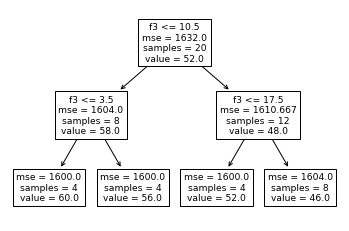
\includegraphics[scale=0.77]{figure1.png}}
\caption{Decision tree building without elimination any features}
\label{fig1}
\end{figure}

If we eliminate the $f_3$ feature from the dataset and apply the same CART procedure, we get a completely different decision tree (fig. 2) that can explain a significantly larger fraction of the variance: $\texttt{score}(\texttt{CART}(f_1, f_2)) = 0.9804$. 


\begin{figure}[htbp]
\centerline{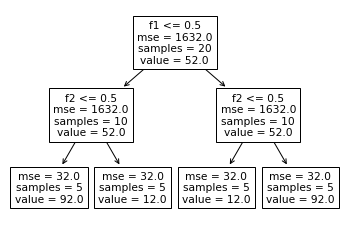
\includegraphics[scale=0.77]{figure2.png}}
\caption{Decision tree building on two complementary features}
\label{fig2}
\end{figure}


As we will see below, the $f_3$ feature is a relatively strong predictor of the target variable, while the $f_1$ and $f_2$ features are weak predictors separately, so if the $f_3$ feature is not excluded from the dataset, it will "overshadow" the $f_1$ and $f_2$ features and not let any of them appear in the decision tree. On the contrary, if $f_3$ is excluded from the dataset, it turns out that $f_1$ and $f_2$ together turn out to be able to significantly increase the fraction of the explained dispersion -- $52.63$ times.


Let us consider the predictive forces of $f_1$, $f_2$ and $f_3$ in more detail. 


Let's consider what is Spearman's correlation of features with the target variable on the whole dataset. Simple calculations show that $f_1$ and $f_2$ do not correlate statistically significantly with the target variable. On the contrary, the $f_3$ feature has a negative correlation of $\rho=-0.49$ ($p$-value $=0.027$). From this we can assume that on the whole dataset $f_3$ is a much stronger predictor than $f_1$ and $f_2$. Obviously, the CART method does not use correlation when choosing an optimal split, but it does not change the conclusions about the strength of predictors. Therefore, the decision tree built by the CART method on a full dataset with all three features consists only of $f_3$ features. That is, at each stage of selecting the optimal split, only feature $f_3$ split wins.


Moreover, it can be shown that on all subsets, which are obtained by splitting the feature $f_1$, there will be no statistically significant correlation between the feature $f_1$ and the target variable. That is, we cannot point to a subset where $f_1$ is a strong predictor by the value of feature $f_1$. The same is true for feature $f_2$.


But if we can't point by the value of the feature itself to a subset where it is positively or negatively correlated with the target variable, then maybe we can point to that subset by the value of another feature? Consider a subset of the analyzed dataset where $f_1=1$. On this subset, Spearman's correlation feature $f_2$ with target $\rho = 0.87$ ($p$-value $ = 0.001$). While the feature $f_3$ correlation is $\rho = -0.49$ ($p$-value $ = 0.14$). We see that the value of feature $f_1$ indicates a subset where $f_2$ has a significantly stronger predictor than $f_3$ and $f_2$ has a greater positive correlation. 


Let us consider the subset of the analyzed dataset, where $f_1=0$. On this subset, Spearman correlation feature $f_2$ with target $\rho = -0.87$ ($p$-value $ = 0.001$). While the f3 feature correlation is the same, po = -0.49 (p-value = 0.14). We see that the feature $f_1$ value indicates a subset where $f_2$ is a significantly stronger predictor than $f_3$ and $f_2$ has a strong negative correlation. 


It turns out that on one subset $f_2$ is strongly positively correlated with target, and on another subset -- strongly negative correlated. And these subsets are specified by the values of $f_1$ feature. By definition, we have that feature $f_1$ is complementary to feature $f_2$. By the same calculation, we can show that feature $f_2$ is complementary to $f_1$. This means that we have reason to believe that if the splits on these features are present together in the same decision tree chain, it is possible that the predictive power of this tree will be greatly higher. We cannot know this for sure, since CART does not use correlation calculation directly, but the complementarity of the feature is a clear signal to test the predictive power of a tree that has these features together in the split in each chain. 

In order for CART to "test" such a decision tree, it is necessary to exclude the $f_3$ feature from the dataset, otherwise it will "overshadow" the $f_1$ and $f_2$ features: at each stage of selecting the optimal split, the $f_3$ features will win, preventing the $f_1$ and $f_2$ features from appearing. Above we have seen that this is exactly what happens: the exclusion of $f_3$ feature from the dataset leads to the creation of a decision tree, each chain of which has both $f_1$ and $f_2$ splits, which allows you to explain the fraction of dispersion of the target variable is 58 times greater than without the use of complementary features.


But the question is, what prevents us from going through all combinations of features in order to find the most appropriate pair of features, possibly complementary? Why accumulate information about the complementarities of the features?


Thus, there is now a need to move from a two-part model of "training -- fitting" to a three-part model of "pretraining -- fine-tuning -- fitting" in the construction of regression trees of decision-making within the framework of explained artificial intelligence, similar to what has already been done in the natural processing language, such as the BERT method \cite{BERT}.

\section{Complementary feature and plausibility}

Let's formally define binary relation of feature complementarity $R \subseteq F^2$ on given dataset $D$ for given $p$ and $\gamma < 0,$   where $F = \{f_i\}$  -- set of features, $p - p$-value, $\gamma - $threshold for the production of correlations given by function \texttt{CorrMul} that defined by algorithm below. 
\theoremstyle{definition}
\begin{definition}{Binary relation $R$ of feature complementarity $R = \{(f_1, f_2) \mid \exists\alpha,\beta(\texttt{CorrMul}_{\alpha,\beta}^{D,p}(f_1, f_2) < \gamma)\} $.
}
\end{definition}

\begin{algorithm}
\SetAlgoLined
\KwData{$D - $dataset, $p - $p-value, $\alpha, \beta - $thresholds, $f_1, f_2 - $features}
\KwResult{Production of correlation}

$D_{\alpha} \gets D[D(f_1) < \alpha]$\;
$D_{\beta} \gets D[D(f_1) < \beta]$\;
$\rho_{\alpha}, p_{\alpha} \gets \texttt{Correlation}(D_{\alpha}(f_2), D(t)) $\;
$\rho_{\beta}, p_{\beta} \gets \texttt{Correlation}(D_{\beta}(f_2), D(t)) $\;
\eIf {$p_{\alpha} \leq p$ \textbf{and} $p_{\beta} \leq p$}{
$\rho \gets \rho_{\alpha} \rho_{\beta}$\;
}{
$\rho \gets 0$\;
}

 \Return $\rho$
 \caption{CorrMul}
\end{algorithm}

Let's define formally binary relation of "paired features", because the condition of decision tree plausibility will be formulated in terms of this relation. Let we have binary relation $R$ on set $F$. We know that we can define domain of the binary relation as $\texttt{Dom} R = \{x \mid \exists y ((x, y) \in R)\}$ and range of the binary relation as $\texttt{Im} R = \{y \mid \exists x ((x, y) \in R)\}$. Now we can define set of all element in the given binary relation $\texttt{Elem} R = \texttt{Dom} R \cup \texttt{Im} R$. 

\theoremstyle{definition}
\begin{definition}{Binary relation $R^*$ of "paired features" \\ $R^* = R \cup R^{-1} \cup \{(x, y) \mid x = y= \texttt{Elem} R\}$.
}
\end{definition}


Let we have binary decision tree with two levels. Let one vertex of the first level -- the root -- has feature $x$. Let vertexes of second level have features $y_1$ and $y_2$. Than formulate the condition on features of plausible decision tree.

\begin{remark}{
if $(x, y_1, y_2 \in F  \setminus \texttt{Elem} R) \lor (xR^*y_1 \land xR^*y_2)$ then two-level decision tree with vertex $x, y_1, y_2$ is seems to be plausible. 
}
\end{remark}

In words we can say that two-levels desicion tree seems to be plausible if features in all vertexes are not the elements of complementary binary relation or if features in each two chains in the tree are paired features. Trees on fig.1 and fig.2 are satisfied to this condition.    

\section{Algorithm of building decision tree}

So, we have collected, accumulated information at the entrance -- the binary relation of complementarity on a set of features. What should be the algorithm to find the decision tree with the highest (or acceptable) predictive power on average faster on the basis of this information, compared to random combinations of two pieces each, on which the CART method is executed?


We suggest the following algorithm. First, we look at all of the pairs from the binary relation of complementarity, and for each of these pairs we build a CART solution tree.  If we intend to generate more trees and if we have run out of pairs from the binary relationship, we randomly choose a subset of a set where the number of features is equal to the square root of the total number of features (as in the Random Forrest method) and for that set of features we build a solution tree. Then we generate a new random subset of the set and build a tree for it, and so on until the total number of built trees will not be required.


Then from the constructed trees we choose the decision tree with the greatest predictive power. It seems quite natural that if the formed relation of complementarity contains rather many pairs of features and the decision tree constructed on complementary features will really often essentially be ahead of predictor's power, then with use of the described algorithm the optimum decision tree will be created faster, than at random selection of pairs of features. But for a quantitative estimation of the advantage in the speed of generation of the optimal tree it will be necessary to conduct additional research. So far, on the above synthetic dataset, with the available information that the $f_1$ and $f_2$ features are complementary to each other, the optimal tree is built at the first attempt, but in case of a random search we have to go through a maximum of 3 variants. It is clear that the advantage of the algorithm over the random search will grow with the increase in the number of features and the extension of the binary relation.

\begin{algorithm}
\SetAlgoLined
\KwData{$d - $dataset, $R - $complementary binary relation, $m - $maximum number of trees}
\KwResult{Optimal decision tree}
 $f \gets$ \texttt{getNumOfFeatures}($d$)\;
 
 \eIf{$m > \abs{R}$}{
   $n \gets m - \abs{R}$\;
   }{
   $n \gets 0$\;
  }
 
 $T \gets \emptyset$\;
 \ForEach {$r \in R$}{
  $F \gets$ \texttt{getFeaturesIDs}($r$)\;
  $t \gets$ \texttt{CART}$_d$($F$)\; 
  $T \gets T \cup \{t\}$\;
 }
 \For {$i = 1$ \KwTo $n$}{
  $F \gets$ \texttt{RandomSet}$\left( \left[\sqrt{f}\right], f \right) $\;
  $t \gets$ \texttt{CART}$_d$($F$)\;
  $T \gets T \cup \{t\}$\;
 }
 
 $k \gets \arg\max_i$ \texttt{Score}($T_i$)\;
 \Return $T_k$
 
 \caption{Decision Tree with Complem. Features}
\end{algorithm}

\section{Discussions}

This paper \cite{mlsd2020} analyzes the relationship between the RISC (Russian index of scientific citations) science metrics and the number of Web of Science (WoS) citations for different groups of researchers. It is shown, that for researchers of "average tier" the greatest correlation with number of citations on WoS from indicators in RISC has the average impact factor of magazines in which the papers are published. This is an argument in favor of the fact that such researchers should focus more on the quality of papers than on the quantity, if their goal -- high citations by WoS. It is also demonstrated that for such researchers the number of articles in Russian journals (including those from the list of the Higher Attestation Commission) has a negative correlation with the number of citations by WoS. This can be interpreted as follows: it is not reasonable for beginners and researchers of the "middle echelon" to focus on an excessive increase in the number of publications in Russian journals that are not part of the RISC core, as this may lead to a move away from the creation of articles that can gain international acceptance.


In terms of complementariry we can say that the feature "number of articles in the core of RISC" and the feature "number of the articles in all Russian scientific magazines" are complementary by definition. That's because value of the first feature can point to the subsets on which second feature correlate with target value in different manner: for one subset correlation is positive, for other -- negative. That's the signal not to use second feature without first feature in decision trees, in estimating researcher. It's an example of applying features complementariry on natural datasets in real tasks. But approbation the idea of building decision trees with using complementary features should proceed further. 

\begin{thebibliography}{00}
\bibitem{mlsd2020} S. A. Saltykov, ``Correlation of scientometric indicators from the RISC with citations based on Web of Science,'' MLSD 2020, in press.
\bibitem{cart} Breiman, Leo; Friedman, J. H.; Olshen, R. A.; Stone, C. J. (1984). ``Classification and regression trees''. Monterey, CA: Wadsworth and Brooks/Cole Advanced Books and Software. ISBN 978-0-412-04841-8.
\bibitem{RF} Ho, Tin Kam (1995). ``Random Decision Forests''. Proceedings of the 3rd International Conference on Document Analysis and Recognition, Montreal, QC, 14–16 August 1995. pp. 278–282.
\bibitem{BERT} Devlin, Jacob, et al. "Bert: Pre-training of deep bidirectional transformers for language understanding." arXiv preprint arXiv:1810.04805 (2018).
\end{thebibliography}

\end{document}
